\section{Packet transactions}
\label{s:transactions}

\begin{figure*}[!t]
\begin{subfigure}{0.5\textwidth}
\begin{small}
\begin{lstlisting}[style=customc]
#define NUM_FLOWLETS    8000
#define THRESHOLD       5
#define NUM_HOPS        10

struct Packet {
  int sport;
  int dport;
  int new_hop;
  int arrival;
  int next_hop;
  int id; // array index
};

int last_time [NUM_FLOWLETS] = {0};
int saved_hop [NUM_FLOWLETS] = {0};

void flowlet(struct Packet pkt) {
  pkt.new_hop = hash3(pkt.sport,
                      pkt.dport,
                      pkt.arrival)
                % NUM_HOPS;

  pkt.id  = hash2(pkt.sport,
                  pkt.dport)
            % NUM_FLOWLETS;

  if (pkt.arrival - last_time[pkt.id] @\label{line:ifStart}@
      > THRESHOLD)
  { saved_hop[pkt.id] = pkt.new_hop; } @\label{line:ifEnd}@

  last_time[pkt.id] = pkt.arrival;
  pkt.next_hop = saved_hop[pkt.id];
}
\end{lstlisting}
\end{small}
\caption{Flowlet switching written in \pktlanguage}
\label{fig:flowlet_code}
\end{subfigure}
%
%
\begin{subfigure}{0.4\textwidth}
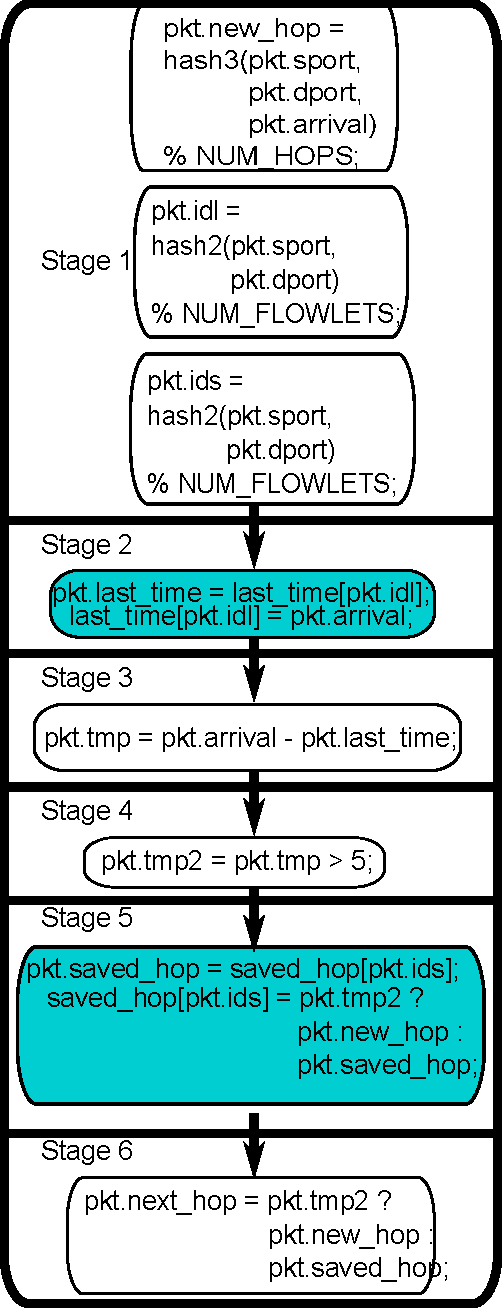
\includegraphics[width=0.9\columnwidth]{pipe.pdf}
\caption{6-stage \absmachine pipeline for flowlet
switching.  Control flows from top to bottom. Stateful atoms are in grey.}
\label{fig:flowlet_pipeline}
\end{subfigure}
\caption{Programming flowlet switching in \pktlanguage}
\end{figure*}

To program a data-plane algorithm, a programmer would write code in
\pktlanguage using packet transactions (Figure~\ref{fig:flowlet_code})
and then use the \pktlanguage compiler to compile to an atom pipeline
for a \absmachine machine (Figure~\ref{fig:flowlet_pipeline}). We
first describe packet transactions in greater detail by walking
through an example (\S\ref{ss:flowlet}). Next, we discuss constraints
in \pktlanguage (\S\ref{ss:constraints}) informed by the domain of
line-rate switches. We then discuss triggering packet transactions
(\S\ref{ss:guards}) and handling multiple transactions
(\S\ref{ss:multiple}).

\subsection{\pktlanguage by example}
\label{ss:flowlet}

We use flowlet switching~\cite{flowlets} as an example. Flowlet
switching is a load-balancing algorithm that sends bursts of packets
(called flowlets) from a TCP flow on different paths, provided the
bursts are separated by a large enough time interval to ensure packets
do not arrive out of order at a TCP
receiver. Figure~\ref{fig:flowlet_code} shows flowlet switching in
\pktlanguage. For simplicity, we hash only the source and destination
ports; it is easy to extend it to the full 5-tuple.

This example demonstrates the core language constructs in
\pktlanguage. All packet processing happens in the context of a packet
transaction (the function \texttt{flowlet} starting at line 17). The
function's argument type {\tt Packet} declares the fields in a packet (lines
5--12)\footnote{We use fields to refer to both packet headers such as
  source port ({\tt sport}) and destination port ({\tt dport}) and
  packet metadata ({\tt id}).} that can be referenced by the function
body (lines 18--32).  The function body can also modify persistent
switch state using global variables (e.g.  \texttt{last\_time} and
\texttt{saved\_hop} on lines 14 and 15, respectively).

Conceptually, the switch invokes the packet transaction function one packet at
a time, with no concurrent packet processing. To the programmer, the function
modifies the passed-in packet argument and runs to completion before processing
the next packet.  The function may invoke \textit{intrinsics} such as
\texttt{hash2} on line 23 to use hardware accelerators such as hash generators.
The \pktlanguage compiler uses an intrinsic's signature to infer dependencies
and supplies a canned run-time implementation, but otherwise does not analyze
an intrinsic's internal behavior. When compiled to a \absmachine machine, the
compiler converts the code in Figure~\ref{fig:flowlet_code} to the atom
pipeline in Figure~\ref{fig:flowlet_pipeline}.

\subsection{Constraints on the language}
\label{ss:constraints}

The syntax of Domino is similar to C, but with several constraints
(Table~\ref{tab:restrict}).  These constraints are required for deterministic
performance.  Memory allocation, unbounded iteration counts, and unstructured
control flow all cause variable performance, which may prevent an algorithm
from achieving line rate.  Additionally, \pktlanguage constrains array
modifications by requiring that all accesses to a given array within one
execution of a transaction, i.e. one packet, must use the same array index. For
example, all read and write accesses to the array \texttt{last\_time} use the
index \texttt{pkt.id}, which is constant for each packet, but can change
between packets. This restriction mirrors restrictions on memories, which don't
typically support distinct read and write addresses every clock cycle.

\begin{table}
  \begin{tabular}{p{0.9\columnwidth}}
    No iteration (while, for, do-while).\\
    No goto, break, or continue.\\
    No pointers.\\
    No dynamic memory allocation / heap.\\
    Array index is constant for each transaction execution.\\
    No access to data i.e. unparsed portion of the packet.\\
  \end{tabular}

  \caption{Restrictions in \pktlanguage}

  \label{tab:restrict}
\end{table}

\subsection{Triggering packet transactions}
\label{ss:guards}
Packet transactions specify \textit{how} to process packet headers and/or
state.  To specify {\em when} to run packet transactions, we provide a {\em
guard}: a predicate on packet fields that triggers the transaction whenever a
packet matches the guard. An example guard (pkt.tcp\_dst\_port == 80) would execute
heavy-hitter detection on all packets on TCP destination port 80. This guard can
be implemented using an exact match in a match-action table, with the actions
being the atoms resulting from compiling the packet transaction. Guards can be of various forms,
e.g., exact, ternary, longest-prefix and range-based matches, depending on the
match semantics supported by the match-action pipeline. Because guards map
rather straightforwardly to the match key in a match-action table, this paper only
focuses on compiling packet transactions.

\subsection{Handling multiple transactions}
\label{ss:multiple}
So far, we have discussed a single packet transaction corresponding to a single
data-plane algorithm. In practice, a switch
would run multiple data-plane algorithms---each processing its own subset of
packets. To accommodate multiple transactions, we envision a policy
language that specifies pairs of guards and transactions. Realizing a policy is
straightforward when all guards are disjoint. When guards overlap, multiple
transactions need to execute on the same subset of packets, requiring a
mechanism to compose transactions. One semantics for composition is to concatenate the two
transaction bodies in an order specified by the user, providing the illusion of
a larger transaction that combines two transactions. We leave a detailed
exploration of this and alternative semantics to future work,
and focus only on compiling a single packet transaction.
